% Straight up stealing preamble from Eli Holmes 
%%%%%%%%%%%%%%%%%%%%%%%%%%%%%%%%%%%%%%START PREAMBLE THAT IS THE SAME FOR ALL EXAMPLES
\documentclass{article}

%Required: You must have these
\usepackage{Sweave}
\usepackage{graphicx}
\usepackage{tabularx}
\usepackage{hyperref}
\usepackage{natbib}
\usepackage{pdflscape}
\usepackage{array}
\usepackage{gensymb}
%\usepackage[backend=bibtex]{biblatex}
%Strongly recommended
  %put your figures in one place
%\SweaveOpts{prefix.string=figures/, eps=FALSE} 
%you'll want these for pretty captioning
\usepackage[small]{caption}

\setkeys{Gin}{width=0.8\textwidth}  %make the figs 50 perc textwidth
\setlength{\captionmargin}{30pt}
\setlength{\abovecaptionskip}{10pt}
\setlength{\belowcaptionskip}{10pt}
% manual for caption  http://www.dd.chalmers.se/latex/Docs/PDF/caption.pdf

%Optional: I like to muck with my margins and spacing in ways that LaTeX frowns on
%Here's how to do that
 \topmargin -1.5cm        
 \oddsidemargin -0.04cm   
 \evensidemargin -0.04cm  % same as oddsidemargin but for left-hand pages
 \textwidth 16.59cm
 \textheight 21.94cm 
 %\pagestyle{empty}       % Uncomment if don't want page numbers
 \parskip 7.2pt           % sets spacing between paragraphs
 %\renewcommand{\baselinestretch}{1.5} 	% Uncomment for 1.5 spacing between lines
\parindent 0pt% sets leading space for paragraphs
\usepackage{setspace}
%\doublespacing

%%%%%%%%%%%%%%%%%%%%%%%%%%%%%%%%%%%%%%END PREAMBLE THAT IS THE SAME FOR ALL EXAMPLES

%Start of the document
\begin{document}

\bibliographystyle{/Users/aileneettinger/citations/Bibtex/styles/amnat.bst}
\title{Supplemental Materials for: How do climate change experiments actually change climate?} % Paper 1/Large group paper from Reconciling Experimental and Observational Approaches for Climate Change Impacts

\author{A.K. Ettinger, I. Chuine, B. Cook, J. Dukes, A.M. Ellison, M.R. Johnston, A.M. Panetta,\\ C. Rollinson, Y. Vitasse, E. Wolkovich}
%\date{\today}
\maketitle  %put the fancy title on
%\tableofcontents      %add a table of contents
%\clearpage
%%%%%%%%%%%%%%%%%%%%%%%%%%%%%%%%%%%%%%%%%%%%%%%%%%%
\renewcommand{\thetable}{S\arabic{table}}
\renewcommand{\thefigure}{S\arabic{figure}}

\section* {Additional methods for database development}
For our literature review, we searched the Web of Science (ISI) for Topic=(warm* OR temperature*) AND Topic=(plant* AND phenolog*) AND Topic=(experiment* OR manip*). We restricted dates to the time period after the STONE database (i.e. January 2011 through March 2015). This yielded 277 new studies. We removed all passive warming studies from the list, and contacted authors for daily data. The resulting database contains daily climate data collected between 1991 and 2014 from North American and European climate change experiments (Table S1, Figure S1). 

\section* {Details of Statistical Analyses and Results}
For all analyses, we use mixed-effects models implemented using the lme4 package in R, version 3.2.4 \citep{bates2015,rcoreteam2016}. Mixed-effects models, also called multi-level or hierarchical models, can account for structured data that violate the independence assumption of traditional linear regression \citep{gelman2007}. In our analyses, we use levels/groupings of experimental site, year, and day of year (doy) to account for this mutual dependence among datapoints. To test for significance of fixed effects in our models, we use Type II tests for models including only main effects and Type III tests for models including interactions, as well as main effects. 
\subsection* {Analysis of effects of time and space on local experimental climate}
To test how treatment effects vary spatially (i.e., among blocks within a study) and temporally (i.e., among years within a study), we used data from the four studies in the C3E database that used blocked designs. We fit linear mixed-effect models with mean daily soil temperature, minimum daily air temperature, and maximum daily air temperature as response predictors (Figure 3 in the main text). For temporal models, we included fixed effects of temperature treatment, year, and their interaction; random effects were site and block nested within site (intercept-only structure, Table \ref{table:blocks_time}). For spatial models, we included fixed effects of temperature treatment, block, and their interaction; random effects were site and year nested within site (intercept-only structure, Table \ref{table:blocks_space}). Both of these models excluded data from plots with precipitation treatments. 
\subsection* {Analysis of effects of infrastructure on local experimental climate}
To test how infrastructure affects local climate, we compared temperature and soil moisture data from the studies in the C3E database that monitored climate in two types of control plots: structural controls (i.e., `shams' or `disturbance controls,'
which contained all the warming infrastructure, such as soil cables or infrared heating units but with no heat
applied) and ambient controls with no infrastructure added. These five studies occurred at two sites: Duke Forest and Harvard Forest \citep{farnsworth1995,clark2014a,marchin2015,pelini2011}. We fit linear mixed effects models by month with mean daily soil temperature, minimum and maximum daily air and soil temperature (\citet{farnsworth1995} did not measure these predictors so there are only four different studies in these models), and soil moisture as response predictors. The fixed explanatory predictor was control type (sham or ambient). To allow for both mean differences in temperature and the effect of control to to vary among sites and years, random effects were site and year nested within site, modeled with a random slopes and random intercepts structure. 
We found that experimental structures altered above-ground and soil temperatures in opposing ways: above-ground temperatures were higher in the structural controls, compared with ambient conditions with no structures installed, whereas soil temperatures were lower in the structural controls compared with ambient soil (Figure 4 in the main text).  In addition, soil moisture was lower in
structural controls compared with ambient conditions. These general patterns were consistent across the different temperature models we fit (mean,
minimum, and maximum soil and air temperatures), although the magnitude varied across months, as well as among studies. We show summaries from models fit to the entire year (Tables \ref{table:shamamb_soiltemp}, \ref{table:shamamb_airtemp}, \ref{table:shamamb_soilmois}), as well as summaries from models fit to each month of data, as is shown in Figure 4 in the main text (Tables \ref{table:shamamb_stempm}, \ref{table:shamamb_atempm}, \ref{table:shamamb_soilmoism}).
\subsection* {Analysis of effects of precipitation treatments on above-ground temperature}
Of the twelve experiments in the C3E database, four manipulated precipitation and measured above-ground temperature. To examine the effects of precipitation treatment on above-ground temperature, we fit linear mixed effect models to data from these four sites with above-ground temperature (daily minimum and maximum) as the response variables. Predictors were precipitation treatment (a continuous fixed effect, which ranged from 50 to 200 \% of ambient for these four studies), target warming (a continuous fixed effect, which ranged from 0 to 4 \degree C for these four studies), and their interaction. To account for methodological and other differences among site, we included site as a random effect, with year and doy nested within site to account for the non-independent nature of measurements taken on the same day within sites. We used a random intercept model structure, (Table \ref{table:preciptemp}). 
\subsection* {Analysis of effects of experimental warming on soil moisture}
Of the twelve experiments in the C3E database, ten measured and reported soil moisture. To examine the effects of target warming treatment on soil moisture, we fit linear mixed effects models to data from these ten sites, excluding plots with precipitation treatments. We first fit a model with soil moisture as the response and a predictor of target warming (this was a continuous fixed effect, which ranged from 0 to 5.2 \degree C for these 10 studies). To account for methodological and other differences among site, we included site as a random effect, with year and doy nested within site to account for the non-independent nature of measurements taken on the same day within sites.  We used a random slope and intercept model structure, to allow the effect of target warming to vary among sites (Table \ref{table:targsoilmois}). 
\par In addition to testing how experimental warming influenced soil moisture, we also tested how experimental structures influenced soil moisture. We compared the soil moisture measured in structural controls to both ambient controls and warmed plots by fitting a model with categorical fixed effects of ``ambient," ``structural control," and ``warmed."  We again included site as a random effect, with doy nested within site to account for the non-independent nature of measurements taken on the same day within sites, and used a random intercept structure (Table \ref{table:warmsoilmois}). 

\subsection* {Analysis of budburst phenology}
We wanted to investigate how using measured plot-level climate variables, as opposed to target warming, alters estimates of temperature sensitivity. To do this, we fit models to data from the five study sites in the C3E database that recorded above-ground temperature and soil moisture, as well as phenology data (doy of budburst). We first fit a model of target warming only to these data, accounting for non-independence by including species, site, and year nested within site as intercept-only random effects (Table \ref{table:bbmods}). We compared this to a model with mean annual measured above-ground temperature (offset by subtracting the minimum temperature across all studies and plots, to make model intercepts more similar), mean winter (January-March) soil moisture, and their interaction as explanatory variables (with the same random effects structure). To determine which specific above-ground temperature variable to include, we compared AICs of models for with four different temperature variables (mean annual minimum and maximum temperatures, mean January-March minimum and maximum temperatures). The model with mean annual minimum temperature, mean January-March soil moisture, and their interaction provided the best model fit (lowest AIC, highest explained variation, Table \ref{table:bbaic}), so we discuss and interpret that model in the main text, summarize it in Table \ref{table:bbmods}, and present its coefficients in Figure 7. 
\bibliography{/Users/aileneettinger/citations/Bibtex/mylibrary}

\section* {Supplemental Tables} 

\begin{table}[b]
  \caption{\textbf{Sites included in the C3E database}. Experimental sites correspond to the map (Figure 1, main text). We give the study ID, location, source, years of data included, and warming type used in the study. Note that some sites may have multiple sources; however, we list only one here. Note that we were unable to include the following studies because authors declined to share their data or did not respond: \citep{schwartzberg2014,moser2011,caron2015,ellebjerg2008}.}
\begin{footnotesize} 
   \begin{tabular}{| p{1.2cm} | p{5.7cm} | p{3.5cm} | p{1.5cm} | p{2cm} |}
    \hline
  study id & location & source & data years & warming type \\ \hline
    exp01 & Waltham, MA, USA & \cite{hoeppner2012} & 2009-2011 & infrared\\ \hline
    exp02 & Montpelier, France & \cite{morin2010} & 2004 & infrared\\ \hline
    exp03 & Duke Forest, NC, USA & \cite{clark2014a} & 2009-2014 & forced air and soil warming\\ \hline
    exp04 & Harvard Forest, MA, USA & \cite{clark2014a} & 2009-2012 & forced air and soil warming\\ \hline
    exp05 & Jasper Ridge Biological Preserve, CA, USA & \cite{cleland2007} & 1998-2002 & infrared\\ \hline
    exp06 & Rocky Mountain Biological Lab, CO, USA & \cite{dunne2003} & 1995-1998 & infrared\\ \hline
    exp07 & Harvard Forest, MA, USA & \cite{pelini2011} & 2010-2015 & forced air \\ \hline
    exp08 & Harvard Forest, MA, USA & \cite{farnsworth1995} & 1993 & soil warming \\ \hline
    exp09 & Stone Valley Forest, PA, USA & \cite{rollinson2012} & 2009-2010 & infrared \\ \hline
    exp10 & Duke Forest, NC, USA & \cite{marchin2015} & 2010-2013 & forced air \\ \hline
    exp11 & Rocky Mountain Biological Lab, CO, USA & \cite{price1998} & 1991-1994 & infrared\\ \hline
    exp12 & Kessler Farm Field Laboratory, OK, USA & \cite{sherry2007} & 2003 & infrared\\ \hline
     \end{tabular} 
    \end{footnotesize}  
    \end{table}
  
\clearpage

\newcolumntype{L}[1]{>{\raggedright\let\newline\\
\arraybackslash\hspace{0pt}}m{#1}}
\newcolumntype{C}[1]{>{\centering\let\newline\\
\arraybackslash\hspace{0pt}}m{#1}}
\newcolumntype{R}[1]{>{\raggedleft\let\newline\\
\arraybackslash\hspace{0pt}}m{#1}}
\newcolumntype{P}[1]{>{\raggedright\tabularxbackslash}p{#1}}


% latex table generated in R 3.4.2 by xtable 1.8-2 package
% Thu Nov  9 16:07:30 2017
\begin{table}[ht]
\centering
\caption{\textbf{Climate measurement details for sites included in the C3E database.} We give the target warming treatment(s) (\degree C), precipitation treatment(s) (percent of ambient), method of above-ground temperature measurement (with height of measurement, in cm, for air), depth(s) of soil temperature measurement (cm), and depth(s) of soil moisture measurement (cm) used in each study.} 
\label{tab:methods}
\begingroup\footnotesize
\begin{tabular}{|p{0.05\textwidth}|p{0.12\textwidth}|p{0.11\textwidth}|p{0.11\textwidth}|p{0.14\textwidth}|p{0.11\textwidth}|}
  \hline
study & warming treatment(s) & precipitation treatment(s) & above-ground temperature & soil temperature depth(s) & soil moisture depth(s) \\ 
  \hline
exp01 & 1 & 50, 100, 150 & canopy & 2, 10 & 30 \\ 
  exp02 & 1.5 & 70, 100 &   &   & 15, 30 \\ 
  exp03 & 3 &   & air (30) & 10 & 30 \\ 
  exp04 & 3 &   & air (30) & 10 & 30 \\ 
  exp05 & 1.5 & 100, 150 &   & 15 & 15 \\ 
  exp06 & 1.5 &   &   & 12, 25 & 12, 25 \\ 
  exp07 & 1.5-5.5 &   & air (22) & 2, 6 & 30 \\ 
  exp08 & 5 &   &   & 5 &   \\ 
  exp09 & 2 & 100, 120 & surface & 3 & 8 \\ 
  exp10 & 1.5-5.5 &   & air (22) & 2, 6 & 30 \\ 
  exp11 & 1 &   &   & 12 &   \\ 
  exp12 & 4 & 100, 200 & air (14) & 7.5, 22.5 & 15 \\ 
   \hline
\end{tabular}
\endgroup
\end{table}
\clearpage

\newcolumntype{L}[1]{>{\raggedright\let\newline\\
\arraybackslash\hspace{0pt}}m{#1}}
\newcolumntype{C}[1]{>{\centering\let\newline\\
\arraybackslash\hspace{0pt}}m{#1}}
\newcolumntype{R}[1]{>{\raggedleft\let\newline\\
\arraybackslash\hspace{0pt}}m{#1}}
\newcolumntype{P}[1]{>{\raggedright\tabularxbackslash}p{#1}}
% latex table generated in R 3.4.2 by xtable 1.8-2 package
% Thu Nov  9 16:15:30 2017
\begin{table}[ht]
\centering
\caption{\textbf{Summary of linear mixed-effects models of how target warming treatment affects daily temperature range (DTR) for above-ground temperatures, and for mimumim and maximum above-ground temperatures in climate change experiments.} We excluded data from plots with precipitation treatments from these analyses. Estimates (est.) are the intercept and coefficient for target warming from the model; se is the standard error for these estimates. The effect of target warming on observed warming was significant based on Type II Wald $\chi^{2}$ tests of fixed effects for minimum above-ground temperature ($\chi^{2}$=40.95, df=1, p<0.001) and maximum above-ground temperature ($\chi^{2}$=4.63, df=1, p=0.03), but not for DTR ($\chi^{2}$=1.18, df=1, p=0.28).  Random effects were site (n=7) and year nested within site (n=29 year-site combinations), with a random slope and intercept structure. Total number of observations=135,943, and units are \degree C for all three models.} 
\label{table:dtrtemp}
\begingroup\footnotesize
\begin{tabular}{|p{0.19\textwidth}|p{0.05\textwidth}p{0.05\textwidth}|p{0.05\textwidth}p{0.05\textwidth}|p{0.05\textwidth}p{0.05\textwidth}|}
  \hline
  &\multicolumn{2}{c |}{DTR} &\multicolumn{2}{c |}{min above-ground temp.} &\multicolumn{2}{c |}{max above-ground temp.}\\
 \hline predictor & est. & se & est. & se & est. & se\\
 \hline
intercept & 14.01 & 1.61 & 5.97 & 0.91 & 20.12 & 1.78 \\ 
  target warming effect & -0.38 & 0.35 & 0.84 & 0.13 & 0.50 & 0.23 \\ 
   \hline
\end{tabular}
\endgroup
\end{table}% latex table generated in R 3.4.2 by xtable 1.8-2 package
% Thu Nov  9 16:15:40 2017
\begin{table}[ht]
\centering
\caption{\textbf{Analysis of variance table for temporal linear mixed-effects models of daily mean soil temperature, minimum above-ground temperature, and maximum above-ground temperature}, fit by maximum likelihood. See Figure 3 in the main text. We list degrees of freedom (which are identical across response variables), test statistics, and p-values for Type III Wald $\chi^{2}$ tests of fixed effects in the models. For all models, random effects were site (n=4 for soil temperature model, n=3 for above-ground temperature models) and block nested within site (intercept-only structure; n=18 for soil, n=12 for above-ground); total number of observations=36,813 for soil and 28,875 for above-ground; units are \degree C.} 
\label{table:blocks_time}
\begingroup\footnotesize
\begin{tabular}{|p{0.20\textwidth}|p{0.01\textwidth}|p{0.09\textwidth}p{0.06\textwidth}|p{0.09\textwidth}p{0.06\textwidth}|p{0.09\textwidth}p{0.06\textwidth}|}
  \hline
  & &\multicolumn{2}{c |}{mean soil temp.} &\multicolumn{2}{c |}{min above-ground temp.} &\multicolumn{2}{c |}{max above-ground temp.}\\
 \hline predictor & df & $\chi^{2}$ & p & $\chi^{2}$ & p & $\chi^{2}$ & p\\
 \hline
intercept & 1 & 126.02 & <0.001 & 24.07 & <0.001 & 233.1 & <0.001 \\ 
  temp. treatment & 4 & 634.87 & <0.001 & 248.69 & <0.001 & 28.95 & <0.001 \\ 
  year & 4 & 325.55 & <0.001 & 327.74 & <0.001 & 318.75 & <0.001 \\ 
  temp. treatment:year & 12 & 196.77 & <0.001 & 126.41 & <0.001 & 188.95 & <0.001 \\ 
   \hline
\end{tabular}
\endgroup
\end{table}% latex table generated in R 3.4.2 by xtable 1.8-2 package
% Thu Nov  9 16:15:45 2017
\begin{table}[ht]
\centering
\caption{\textbf{Analysis of variance table for spatial linear mixed-effects models of daily mean soil temperature, minimum above-ground temperature, and maximum above-ground temperature}, fit by maximum likelihood. See Figure 3 in the main text. We list degrees of freedom (which are identical for all models), test statistics, and p-values for Type III Wald $\chi^{2}$ tests of fixed effects in the models. For all models, random effects were site (n=6) and year nested within site (intercept-only structure; n=6); total number of observations=17,177.} 
\label{table:blocks_space}
\begingroup\footnotesize
\begin{tabular}{|p{0.23\textwidth}|p{0.01\textwidth}|p{0.09\textwidth}p{0.06\textwidth}|p{0.09\textwidth}p{0.06\textwidth}|p{0.09\textwidth}p{0.06\textwidth}|}
  \hline
  & &\multicolumn{2}{c |}{mean soil temp.} &\multicolumn{2}{c |}{min above-ground temp.} &\multicolumn{2}{c |}{max above-ground temp.}\\
 \hline predictor & df & $\chi^{2}$ & p & $\chi^{2}$ & p & $\chi^{2}$ & p\\
 \hline
intercept & 1 & 334.9 & <0.001 & 48.23 & <0.001 & 419.45 & <0.001 \\ 
  temp. treatment & 4 & 382.31 & <0.001 & 215.06 & <0.001 & 83.03 & <0.001 \\ 
  block & 5 & 17.43 & 0.004 & 60.13 & <0.001 & 44.45 & <0.001 \\ 
  temp. treatment:block & 14 & 149.27 & <0.001 & 75.16 & <0.001 & 173.88 & <0.001 \\ 
   \hline
\end{tabular}
\endgroup
\end{table}\clearpage

% latex table generated in R 3.4.2 by xtable 1.8-2 package
% Thu Nov  9 16:16:39 2017
\begin{table}[ht]
\centering
\caption{\textbf{Summaries of linear mixed-effects models comparing effects of ambient versus structural controls on daily mean, minimum, and maximum soil temperature in climate change experiments across the year}. Estimates (est.) are the intercept (representing ambient controls) and coefficient (representing structure effects) from the models; se is the standard error for these estimates. For these annual models, differences between control types were significant based on Type II Wald $\chi^{2}$ tests of fixed effects for mean soil temperature ($\chi^{2}$=5.53, df=1, p=0.02) and minimum soil temperature ($\chi^{2}$=3.87, df=1, p=0.05), but not for maximum soil temperature ($\chi^{2}$=2.07, df=1, p=0.15). For all models, random effects of site (n=5 for mean model, n=4 for min and max models) and year nested within site (n=21 for mean model, n=20 for min and max models) were fit with a random slope and intercept structure; total number of observations= 48,860 for the mean model and 44,530 for the min and max models; units are \degree C.} 
\label{table:shamamb_soiltemp}
\begingroup\footnotesize
\begin{tabular}{|p{0.15\textwidth}|p{0.05\textwidth}p{0.05\textwidth}|p{0.05\textwidth}p{0.05\textwidth}|p{0.05\textwidth}p{0.05\textwidth}|}
  \hline
  &\multicolumn{2}{c |}{mean soil temp.} &\multicolumn{2}{c |}{min soil temp.} &\multicolumn{2}{c |}{max soil temp.}\\
 \hline predictor & est. & se & est. & se & est. & se\\
 \hline
intercept & 11.89 & 1.42 & 10.81 & 1.48 & 13.92 & 1.61 \\ 
  structure effect & -0.57 & 0.24 & -0.63 & 0.32 & -0.54 & 0.38 \\ 
   \hline
\end{tabular}
\endgroup
\end{table}
% latex table generated in R 3.4.2 by xtable 1.8-2 package
% Thu Nov  9 16:16:40 2017
\begin{table}[ht]
\centering
\caption{\textbf{Summaries of linear mixed-effects models comparing effects of ambient versus structural controls on daily minimum and maximum air temperature in climate change experiments, across the year.} Estimates (est.) are the intercept (representing ambient controls) and coefficient (representing structure effects) from the models; se is the standard error for these estimates. For these annual models, differences between control types were not significant based on Type II Wald $\chi^{2}$ tests of fixed effects for minimum air temperature ($\chi^{2}$=1.07, df=1, p=0.30), nor for maximum air temperature ($\chi^{2}$=0.01, df=1, p=0.91). For both models, random effects of site (n=4) and year nested within site (n=20) were fit with a random slope and intercept structure; total number of observations= 44,085; units are \degree C.} 
\label{table:shamamb_airtemp}
\begingroup\footnotesize
\begin{tabular}{|p{0.13\textwidth}|p{0.05\textwidth}p{0.05\textwidth}|p{0.05\textwidth}p{0.05\textwidth}|}
  \hline
  &\multicolumn{2}{c |}{min air temp.} &\multicolumn{2}{c |}{max air temp.}\\
 \hline predictor & est. & se & est. & se\\
 \hline
intercept & 6.29 & 1.51 & 17.74 & 1.81 \\ 
  structure effect & 0.36 & 0.35 & 0.02 & 0.21 \\ 
   \hline
\end{tabular}
\endgroup
\end{table}
% latex table generated in R 3.4.2 by xtable 1.8-2 package
% Thu Nov  9 16:16:50 2017
\begin{table}[ht]
\centering
\caption{\textbf{Summary of a linear mixed-effects model comparing effects of ambient versus structural controls on daily soil moisture (\% volumetric water content, VWC) in climate change experiments across the year.} Estimates (est.) are the intercept (representing ambient controls) and coefficient (representing structure effects) from the models; se is the standard error for these estimates. For this annual model, the difference between control types was significant based on Type II Wald $\chi^{2}$ tests of fixed effects ($\chi^{2}$=89.95, df=1, p<0.001). Random effects of site (n=5) and year nested within site (n=21 year-site combinations) were fit with a random slope and intercept structure; total number of observations= 44,468.} 
\label{table:shamamb_soilmois}
\begingroup\footnotesize
\begin{tabular}{|p{0.18\textwidth}|p{0.16\textwidth}|p{0.05\textwidth}|}
  \hline
  &\multicolumn{2}{c |}{soil moisture (vwc)}\\
 \hline predictor & est. & se\\
 \hline
intercept & 21.20 & 1.86 \\ 
  structure effect & -2.43 & 0.26 \\ 
   \hline
\end{tabular}
\endgroup
\end{table}\clearpage
%monthly models for soil temperature
% latex table generated in R 3.4.2 by xtable 1.8-2 package
% Thu Nov  9 16:17:21 2017
\begin{table}[ht]
\centering
\caption{\textbf{Summaries of linear mixed-effects models, fit to each month of data, comparing effects of ambient versus structural controls on daily mean, minimum, and maximum soil temperature, fit to each month separately}, consistent with Figure 4 in the main text. Estimates (est.) are the intercept (representing ambient controls) and coefficient (representing structural effects) from the models; se is the standard error for these estimates. We list test statistics, and p-values for Type II Wald $\chi^{2}$ tests of fixed effects (df=1 for all tests). Random effects of site (n=5 for all mean soil temperature models; n=4 for all min and max soil temperature models) and year nested within site (n=19 or 20 year-site combinations for all mean soil temperature models; n=18 or 19 for all min and max soil temperature models) were fit with a random slope and intercept structure; total number of observations ranged from 3,814 to 4,186; units are \degree C.} 
\label{table:shamamb_stempm}
\begingroup\footnotesize
\begin{tabular}{|p{0.02\textwidth}|p{0.12\textwidth}|p{0.04\textwidth}p{0.03\textwidth}p{0.04\textwidth}p{0.05\textwidth}|p{0.04\textwidth}p{0.03\textwidth}p{0.04\textwidth}p{0.05\textwidth}|p{0.04\textwidth}p{0.03\textwidth}p{0.04\textwidth}p{0.05\textwidth}|}
  \hline
  & &\multicolumn{4}{c |}{mean soil temp.} &\multicolumn{4}{c |}{min soil temp.} &\multicolumn{4}{c |}{max soil temp.}\\
 \hline mon & predictor & est. & se & $\chi^{2}$ & p & est. & se & $\chi^{2}$ & p & est. & se & $\chi^{2}$ & p\\
 \hline
01 & intercept & 2.66 & 1.25 & 3.63 & 0.057 & 2.34 & 1.21 & 2.09 & 0.149 & 3.92 & 1.65 & 13.71 & <0.001 \\ 
    & structure effect & -0.45 & 0.23 &  &  & -0.72 & 0.50 &  &  & -0.35 & 0.09 &  &  \\ 
   \hline
02 & intercept & 2.86 & 1.44 & 13.06 & <0.001 & 2.58 & 1.26 & 3.24 & 0.072 & 4.66 & 1.92 & 1.99 & 0.158 \\ 
    & structure effect & -0.44 & 0.12 &  &  & -0.67 & 0.37 &  &  & -0.41 & 0.29 &  &  \\ 
   \hline
03 & intercept & 5.24 & 1.78 & 6.44 & 0.011 & 4.66 & 1.58 & 3.64 & 0.056 & 7.75 & 2.04 & 0.92 & 0.337 \\ 
    & structure effect & -0.44 & 0.17 &  &  & -0.44 & 0.23 &  &  & -0.50 & 0.52 &  &  \\ 
   \hline
04 & intercept & 9.98 & 1.85 & 8.53 & 0.003 & 8.93 & 1.98 & 10.52 & 0.001 & 13.24 & 1.80 & 0.96 & 0.327 \\ 
    & structure effect & -0.67 & 0.23 &  &  & -0.65 & 0.20 &  &  & -0.63 & 0.65 &  &  \\ 
   \hline
05 & intercept & 14.92 & 1.37 & 3.85 & 0.05 & 13.74 & 1.54 & 4.91 & 0.027 & 17.54 & 1.41 & 0.59 & 0.441 \\ 
    & structure effect & -0.31 & 0.16 &  &  & -0.27 & 0.12 &  &  & -0.32 & 0.42 &  &  \\ 
   \hline
06 & intercept & 18.29 & 1.58 & 0 & 0.972 & 17.43 & 1.57 & 0.76 & 0.383 & 20.98 & 1.78 & 0.04 & 0.844 \\ 
    & structure effect & -0.01 & 0.20 &  &  & -0.14 & 0.16 &  &  & 0.09 & 0.47 &  &  \\ 
   \hline
07 & intercept & 21.07 & 1.33 & 0.06 & 0.815 & 19.97 & 1.34 & 0.45 & 0.501 & 23.76 & 1.46 & 0.01 & 0.914 \\ 
    & structure effect & -0.07 & 0.28 &  &  & -0.12 & 0.18 &  &  & -0.07 & 0.61 &  &  \\ 
   \hline
08 & intercept & 20.93 & 1.20 & 2.56 & 0.11 & 19.59 & 1.29 & 1.35 & 0.244 & 23.23 & 1.42 & 1.58 & 0.209 \\ 
    & structure effect & -0.26 & 0.16 &  &  & -0.20 & 0.17 &  &  & -0.37 & 0.30 &  &  \\ 
   \hline
09 & intercept & 18.23 & 1.24 & 10.15 & 0.001 & 16.94 & 1.36 & 0.58 & 0.445 & 20.54 & 1.43 & 1.74 & 0.188 \\ 
    & structure effect & -0.36 & 0.11 &  &  & -0.21 & 0.27 &  &  & -0.40 & 0.31 &  &  \\ 
   \hline
10 & intercept & 13.03 & 1.22 & 10.48 & 0.001 & 12.26 & 1.24 & 1.39 & 0.239 & 15.42 & 1.39 & 10.02 & 0.002 \\ 
    & structure effect & -0.42 & 0.13 &  &  & -0.56 & 0.48 &  &  & -0.50 & 0.16 &  &  \\ 
   \hline
11 & intercept & 8.27 & 1.13 & 1.87 & 0.172 & 7.34 & 1.23 & 0.83 & 0.363 & 10.11 & 1.43 & 3.16 & 0.075 \\ 
    & structure effect & -0.33 & 0.24 &  &  & -0.52 & 0.57 &  &  & -0.28 & 0.16 &  &  \\ 
   \hline
12 & intercept & 5.03 & 1.21 & 2.8 & 0.094 & 4.38 & 1.24 & 1.53 & 0.215 & 6.40 & 1.53 & 4.83 & 0.028 \\ 
    & structure effect & -0.40 & 0.24 &  &  & -0.61 & 0.49 &  &  & -0.26 & 0.12 &  &  \\ 
   \hline
\end{tabular}
\endgroup
\end{table}\clearpage

%monthly air temperature models
% latex table generated in R 3.4.2 by xtable 1.8-2 package
% Thu Nov  9 16:17:39 2017
\begin{table}[ht]
\centering
\caption{\textbf{Summaries of linear mixed-effects models, fit to each month comparing effects of ambient versus structural controls on daily minimum and maximum above-ground temperature, fit to each month separately}, consistent with Figure 4 in the main text. Estimates (est.) are the intercept (representing ambient controls) and coefficient (representing structural effects) from the models; se is the standard error for these estimates. We list test statistics, and p-values for Type II Wald $\chi^{2}$ tests of fixed effects (df=1 for all tests). Random effects of site (n=4 for both models) and year nested within site (n=18 year-site combinations for both models) were fit with a random slope and intercept structure; total number of observations was 3,726; units are \degree C.} 
\label{table:shamamb_atempm}
\begingroup\footnotesize
\begin{tabular}{|p{0.03\textwidth}|p{0.14\textwidth}|p{0.05\textwidth}p{0.04\textwidth}p{0.06\textwidth}p{0.06\textwidth}|p{0.05\textwidth}p{0.04\textwidth}p{0.06\textwidth}p{0.06\textwidth}|}
  \hline
  & &\multicolumn{4}{c |}{min air temp.} &\multicolumn{4}{c |}{max air temp.}\\
 \hline mon & predictor & est. & se & $\chi^{2}$ & p & est. & se & $\chi^{2}$ & p\\
 \hline
01 & intercept & -5.49 & 1.78 & 5.27 & 0.022 & 5.09 & 2.60 & 0.01 & 0.927 \\ 
    & structure effect & 0.61 & 0.26 &  &  & -0.03 & 0.29 &  &  \\ 
   \hline
02 & intercept & -3.92 & 1.83 & 1.41 & 0.235 & 7.10 & 3.03 & 2.93 & 0.087 \\ 
    & structure effect & 0.55 & 0.46 &  &  & 0.36 & 0.21 &  &  \\ 
   \hline
03 & intercept & -0.08 & 1.55 & 8.59 & 0.003 & 12.60 & 2.41 & 2.75 & 0.097 \\ 
    & structure effect & 0.50 & 0.17 &  &  & 0.52 & 0.31 &  &  \\ 
   \hline
04 & intercept & 5.28 & 1.80 & 9.33 & 0.002 & 19.27 & 1.92 & 18.31 & <0.001 \\ 
    & structure effect & 0.55 & 0.18 &  &  & 1.26 & 0.29 &  &  \\ 
   \hline
05 & intercept & 11.62 & 1.46 & 6.56 & 0.01 & 23.49 & 1.03 & 7.75 & 0.005 \\ 
    & structure effect & 0.48 & 0.19 &  &  & 0.77 & 0.28 &  &  \\ 
   \hline
06 & intercept & 15.45 & 1.47 & 10.13 & 0.001 & 26.32 & 1.82 & 4.4 & 0.036 \\ 
    & structure effect & 0.43 & 0.14 &  &  & 0.59 & 0.28 &  &  \\ 
   \hline
07 & intercept & 17.90 & 1.26 & 4.47 & 0.035 & 28.94 & 1.25 & 3.58 & 0.059 \\ 
    & structure effect & 0.85 & 0.40 &  &  & 0.61 & 0.32 &  &  \\ 
   \hline
08 & intercept & 17.07 & 1.43 & 2.07 & 0.15 & 27.39 & 1.15 & 0.87 & 0.35 \\ 
    & structure effect & 0.65 & 0.45 &  &  & 0.33 & 0.35 &  &  \\ 
   \hline
09 & intercept & 13.34 & 1.39 & 4.71 & 0.03 & 23.72 & 1.47 & 2.66 & 0.103 \\ 
    & structure effect & 0.88 & 0.41 &  &  & 0.38 & 0.23 &  &  \\ 
   \hline
10 & intercept & 7.26 & 1.26 & 4.27 & 0.039 & 17.29 & 1.70 & 1.89 & 0.169 \\ 
    & structure effect & 0.79 & 0.38 &  &  & 0.30 & 0.22 &  &  \\ 
   \hline
11 & intercept & 1.21 & 1.25 & 4.23 & 0.04 & 12.79 & 1.83 & 2.76 & 0.097 \\ 
    & structure effect & 0.88 & 0.43 &  &  & 0.26 & 0.15 &  &  \\ 
   \hline
12 & intercept & -2.83 & 1.48 & 5.29 & 0.021 & 7.56 & 2.38 & 0.26 & 0.61 \\ 
    & structure effect & 0.43 & 0.19 &  &  & -0.11 & 0.23 &  &  \\ 
   \hline
\end{tabular}
\endgroup
\end{table}\clearpage

%monthly soil moisture models
% latex table generated in R 3.4.2 by xtable 1.8-2 package
% Thu Nov  9 16:17:48 2017
\begin{table}[ht]
\centering
\caption{\textbf{Summaries of linear mixed-effects models, fit to each month comparing effects of ambient versus structural controls on soil moisture (\% VWC), fit to each month separately}, consistent with Figure 4 in the main text. Estimates (est.) are the intercept (representing ambient controls) and coefficient (representing structural effects) from the models; se is the standard error for these estimates. We list test statistics, and p-values for Type II Wald $\chi^{2}$ tests of fixed effects; df=1 for all models. Random effects of site (n=4) and year nested within site (n=18 year-site combinations) were fit with a random slope and intercept structure; total number of observations was 3,829.} 
\label{table:shamamb_soilmoism}
\begingroup\footnotesize
\begin{tabular}{|p{0.03\textwidth}|p{0.14\textwidth}|p{0.05\textwidth}p{0.04\textwidth}p{0.06\textwidth}p{0.06\textwidth}|}
  \hline
mon & predictor & est. & se & $\chi^2$ & p \\ 
  \hline
01 & intercept & 22.58 & 3.23 & 59.24 & <0.001 \\ 
    & structure effect & -2.77 & 0.36 &  &  \\ 
   \hline
02 & intercept & 22.10 & 3.24 & 16.78 & <0.001 \\ 
    & structure effect & -2.54 & 0.62 &  &  \\ 
   \hline
03 & intercept & 23.58 & 2.43 & 8.3 & 0.004 \\ 
    & structure effect & -2.48 & 0.86 &  &  \\ 
   \hline
04 & intercept & 22.54 & 2.15 & 9.24 & 0.0024 \\ 
    & structure effect & -2.06 & 0.68 &  &  \\ 
   \hline
05 & intercept & 21.08 & 2.31 & 40.17 & <0.001 \\ 
    & structure effect & -2.20 & 0.35 &  &  \\ 
   \hline
06 & intercept & 18.44 & 1.37 & 30.78 & <0.001 \\ 
    & structure effect & -2.12 & 0.38 &  &  \\ 
   \hline
07 & intercept & 17.60 & 2.18 & 20.22 & <0.001 \\ 
    & structure effect & -2.38 & 0.53 &  &  \\ 
   \hline
08 & intercept & 16.59 & 1.90 & 12.95 & <0.001 \\ 
    & structure effect & -2.09 & 0.58 &  &  \\ 
   \hline
09 & intercept & 15.99 & 1.54 & 13.2 & <0.001 \\ 
    & structure effect & -1.79 & 0.49 &  &  \\ 
   \hline
10 & intercept & 20.15 & 1.93 & 20.9 & <0.001 \\ 
    & structure effect & -2.27 & 0.50 &  &  \\ 
   \hline
11 & intercept & 21.18 & 1.77 & 21.9 & <0.001 \\ 
    & structure effect & -2.70 & 0.58 &  &  \\ 
   \hline
12 & intercept & 22.74 & 2.83 & 15.64 & <0.001 \\ 
    & structure effect & -2.88 & 0.73 &  &  \\ 
   \hline
\end{tabular}
\endgroup
\end{table}
%tried deleting from here down to line 650 to see if pdf would compile...wouldn't so problem is probabily below 650
\clearpage
%how do precip treatments affect above-ground temperature
% latex table generated in R 3.4.2 by xtable 1.8-2 package
% Thu Nov  9 16:18:35 2017
\begin{table}[ht]
\centering
\caption{\textbf{Summary of a linear mixed-effects models of how precipitation treatment affects above-ground minimum and maximum temperatures in climate change experiments.} We include data from all studies that manipulated precipitation and measured daily above-ground temperature. Estimates (est.) are the intercept and coefficients for precipitation and warming treatments, as well as their interaction, from the model; se is the standard error for these estimates; p-values represent significance tests for Type III Wald $\chi^{2}$ tests. Random effects were site (n=4), year of study (n=9 year:site combinations), and doy nested within year (n=2599 doy:year:site combinations), with a random intercept structure. Total number of observations was 70463.} 
\label{table:preciptemp}
\begingroup\footnotesize
\begin{tabular}{|p{0.20\textwidth}|p{0.10\textwidth}|p{0.04\textwidth}|p{0.03\textwidth}|p{0.05\textwidth}|p{0.01\textwidth}|p{0.05\textwidth}|}
  \hline
response & predictors & est. & se & $\chi^{2}$ & df & p \\ 
  \hline
min above-ground temp. & intercept & 7.21 & 0.85 & 72.15 & 1 & <0.001 \\ 
   & preciptreat & -0.01 & 0.00 & 952.21 & 1 & <0.001 \\ 
   & target & 0.74 & 0.01 & 4559.82 & 1 & <0.001 \\ 
   & precip*target & 0.00 & 0.00 & 63.80 & 1 & <0.001 \\ 
   \hline
max above-ground temp. & intercept & 23.91 & 1.00 & 574.81 & 1 & <0.001 \\ 
   & preciptreat & -0.02 & 0.00 & 2448.37 & 1 & <0.001 \\ 
   & target & 0.78 & 0.02 & 1876.46 & 1 & <0.001 \\ 
   & precip*target & -0.00 & 0.00 & 30.35 & 1 & <0.001 \\ 
   \hline
\end{tabular}
\endgroup
\end{table}
%how soil  moisture is affected by warming treatment
% latex table generated in R 3.4.2 by xtable 1.8-2 package
% Thu Nov  9 16:18:56 2017
\begin{table}[ht]
\centering
\caption{\textbf{Summary of a linear mixed-effects model of how target warming treatment affects soil moisture  (\% VWC) in climate change experiments.} We excluded data from plots with precipitation treatments from this analysis. Estimates (est.) are the intercept and coefficient for target warming from the model; se is the standard error for these estimates. The effect of target warming was significant, based on Type II Wald $\chi^{2}$ tests of the fixed effect ($\chi^{2}$=3.49, df=2, p=0.06). Random effects were site (n=10), year of study, and doy nested within year (n=2434 doy-site combinations), with a random intercept structure. Total number of observations was 72730.} 
\label{table:targsoilmois}
\begingroup\footnotesize
\begin{tabular}{|p{0.20\textwidth}|p{0.05\textwidth}p{0.05\textwidth}|}
  \hline
 & est. & se \\ 
  \hline
intercept & 20.85 & 1.28 \\ 
  target & -0.36 & 0.01 \\ 
   \hline
\end{tabular}
\endgroup
\end{table}% latex table generated in R 3.4.2 by xtable 1.8-2 package
% Thu Nov  9 16:19:20 2017
\begin{table}[ht]
\centering
\caption{\textbf{Summary of a linear mixed-effects model comparing soil moisture (\% VWC)} in experimentally warmed plots to two different control types, structural and ambient controls. We excluded data from plots with precipitation treatments from this analysis. Estimates (est.) are the intercept (representing mean moisture in ambient controls)  and coefficients from the from the model (i.e. differences between the ambient) for structural controls and warmed plots (pooled across all target warming levels); se is the standard error for these estimates. There were significant differences among warming types based on Type II Wald $\chi^{2}$ tests of the fixed effect ($\chi^{2}$=7229.01, df=2, p<0.001). Random effects were site (n=10), year nested within site (n=35 site-year combinations), and doy nested within year (7,979 doy-year-site combinations) with a random intercept structure. Total number of observations was 72730.} 
\label{table:warmsoilmois}
\begingroup\footnotesize
\begin{tabular}{|p{0.2\textwidth}|p{0.05\textwidth}p{0.05\textwidth}|}
  \hline
 & est. & se \\ 
  \hline
intercept & 22.31 & 1.31 \\ 
  structure effect & -1.93 & 0.04 \\ 
  warmed effect & -2.85 & 0.03 \\ 
   \hline
\end{tabular}
\endgroup
\end{table}%deleted from here to 746 to see if pdf could compile and it could!

%budburst analyses
% latex table generated in R 3.4.2 by xtable 1.8-2 package
% Thu Nov  9 16:19:48 2017
\begin{table}[ht]
\centering
\caption{\textbf{Comparison of linear mixed-effects models for budburst doy} that contain either target warming treatment only as a fixed effect or measured mean annual minimum temperature (\degree C), mean soil moisture from January through March (in \% VWC), and their interaction as fixed effects. Estimates (est.) are the intercept and coefficients from the models; se is the standard error for these estimates. Both models include random effects of site (n=5), year of study nested within site (n=13 year-site combinations), and plant species (n=54), each with a random intercept structure. Total number of observations was 12839.} 
\label{table:bbmods}
\begingroup\footnotesize
\begin{tabular}{|p{0.18\textwidth}|p{0.18\textwidth}|p{0.05\textwidth}|p{0.05\textwidth}|}
  \hline
V1 & predictor & est. & se \\ 
  \hline
target warming model & intercept & 110.06 & 6.95 \\ 
   & target & -2.01 & 0.08 \\ 
   \hline
tmin*soilmois model & intercept & 146.42 & 5.14 \\ 
   & tmin & -6.22 & 0.41 \\ 
   & soilmois\_janmar & -1.35 & 0.12 \\ 
   & tmin*soilmois\_janmar & 0.16 & 0.02 \\ 
   \hline
\end{tabular}
\endgroup
\end{table}% latex table generated in R 3.4.2 by xtable 1.8-2 package
% Thu Nov  9 16:19:48 2017
\begin{table}[ht]
\centering
\caption{\textbf{Comparison of budburst model fits} from four models with different fixed effects: 1) target warming only, 2) measured mean annual minimum temperature (tmin) only, tmin and soil moisture (soilmois), and tmin, soilmois, and their interaction. We additionally compared models with mean annual maximum temperature, and seasonal temperature variables; we present only tmin here because this variable provided the best model fit (i.e. lowest AIC).} 
\label{table:bbaic}
\begingroup\footnotesize
\begin{tabular}{|p{0.18\textwidth}|p{0.02\textwidth}|p{0.08\textwidth}|p{0.05\textwidth}|}
  \hline
model & df & AIC & $\Delta$AIC \\ 
  \hline
tmin*soilmois & 8 & 104752.16 & 0.00 \\ 
  tmin+soilmois & 7 & 104825.61 & 73.45 \\ 
  target & 6 & 104889.13 & 136.97 \\ 
  tmin & 6 & 104903.49 & 151.33 \\ 
   \hline
\end{tabular}
\endgroup
\end{table}\clearpage

\clearpage
\section* {Supplmenetal Figures}
\begin{figure}[p]
\centering
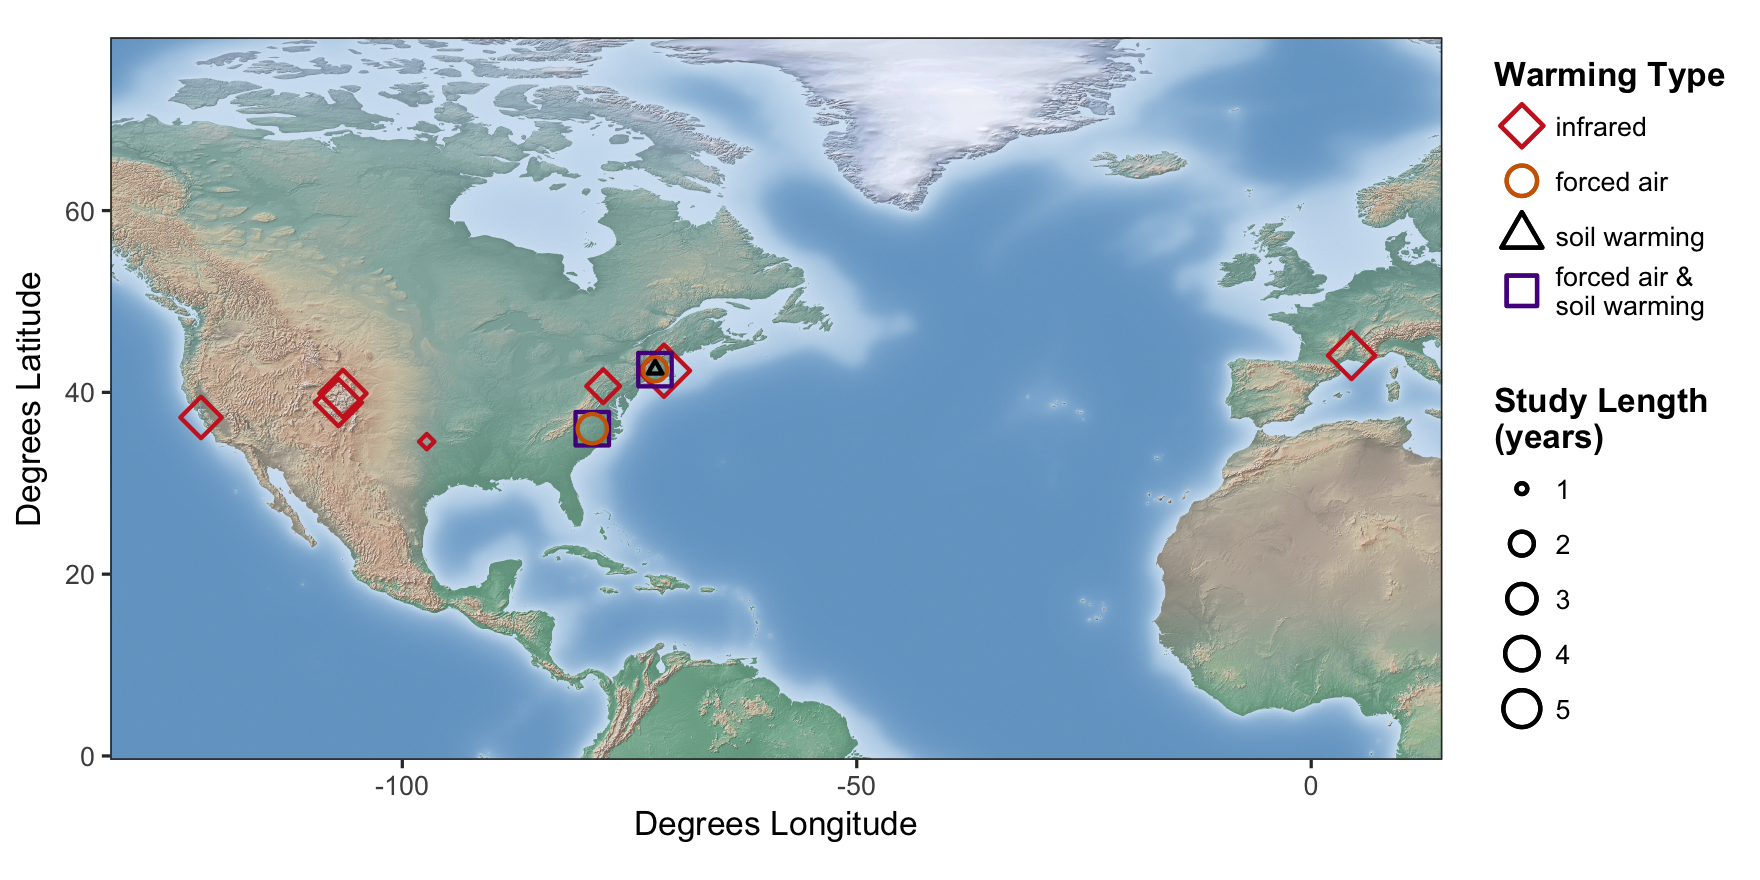
\includegraphics{/Users/aileneettinger/git/radcliffe/Analyses/maps/RadcliffeLocations_Experiments_Open.png} 
\caption{\textbf{Climate data from 12 climate change experiments in North America and Europe are included in the C3E database and analyzed here.} See Tables S1 and S2 for details.} 
 \label{fig:map}
 \end{figure}
\clearpage
\begin{figure}[p]
\centering
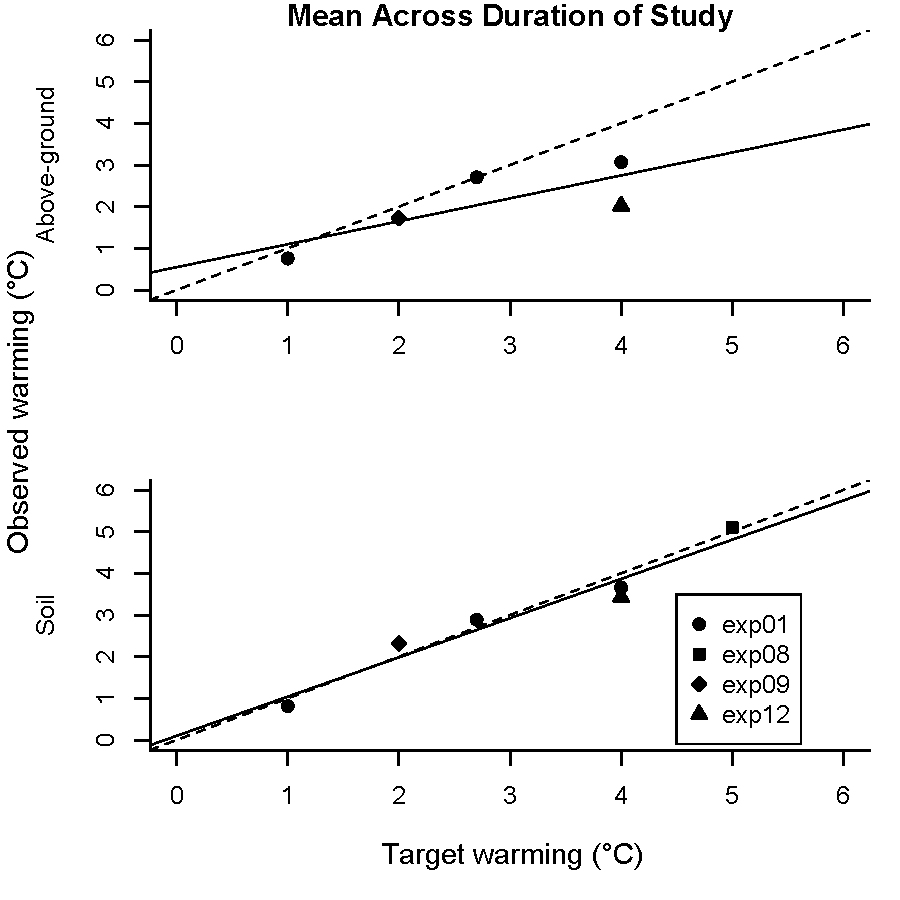
\includegraphics{/Users/aileneettinger/git/radcliffe/Analyses/figures/targetvsobs_stduration.pdf} 
\caption{\textbf{Mean warming across the study duration.} Reporting only the mean temperature difference across the duration of the study, as is commonly done in publications of climate change experiments, hides potentially important variations in daily, seasonal, and annual temperatures among treatments. The solid line is the fitted relationship between observed and target warming and the dashed line shows when observed warming is exactly equal to target warming (1:1). Compare to Figure 2 in the main text. } 
 \label{fig:targetvsobs}
 \end{figure}


%%%%%%%%%%%%%%%%%%%%%%%%%%%%%%%%%%%%%%%%
\end{document}
%%%%%%%%%%%%%%%%%%%%%%%%%%%%%%%%%%%%%%%%
